\documentclass[11pt,a4paper]{article}
\usepackage[margin=2.2cm,headheight=14pt]{geometry}
\usepackage[T1]{fontenc}
\usepackage{lmodern}
\usepackage{microtype}
\usepackage{amsmath,amssymb}
\usepackage{graphicx}
\usepackage{booktabs}
\usepackage{tabularx}
\usepackage{multirow}
\usepackage[table]{xcolor}
\usepackage{enumitem}
\usepackage{caption}
\usepackage[section]{placeins}
\usepackage{titlesec}
\usepackage{fancyhdr}
\usepackage[most]{tcolorbox}
\usepackage[colorlinks,linkcolor=accent,citecolor=accent,urlcolor=accent]{hyperref}

\definecolor{accent}{HTML}{1F4E8C}
\definecolor{accentbg}{HTML}{EEF3FA}

% Headings
\titleformat{\section}{\Large\sffamily\bfseries\color{accent}}{\thesection}{0.6em}{}
\titleformat{\subsection}{\large\sffamily\bfseries\color{accent}}{\thesubsection}{0.6em}{}
\titleformat{\paragraph}[runin]{\normalsize\bfseries}{}{}{}
\titlespacing*{\section}{0pt}{14pt plus 3pt minus 2pt}{6pt plus 2pt}
\titlespacing*{\subsection}{0pt}{10pt plus 2pt minus 2pt}{4pt plus 1pt}
\titlespacing*{\paragraph}{0pt}{6pt plus 2pt minus 1pt}{0.6em}

% Header and footer
\pagestyle{fancy}
\fancyhf{}
\fancyhead[L]{\small\sffamily\color{gray}DSA5208 Project 3 \textperiodcentered\ Distributed PageRank}
\fancyhead[R]{\small\sffamily\color{gray}\nouppercase{\leftmark}}
\fancyfoot[C]{\small\sffamily\thepage}
\renewcommand{\headrulewidth}{0.4pt}
\renewcommand{\sectionmark}[1]{\markboth{\thesection\quad #1}{}}
\fancypagestyle{plain}{\fancyhf{}\renewcommand{\headrulewidth}{0pt}\fancyfoot[C]{\small\sffamily\thepage}}

% Captions, lists, floats
\captionsetup{font=small,labelfont={bf,sf,color=accent},labelsep=period,skip=5pt}
\setlist{itemsep=1pt,topsep=3pt}
\setlength{\textfloatsep}{12pt plus 3pt minus 3pt}
\setlength{\floatsep}{10pt plus 3pt minus 2pt}
\renewcommand{\arraystretch}{1.08}
\renewcommand{\topfraction}{0.85}
\renewcommand{\bottomfraction}{0.6}
\renewcommand{\textfraction}{0.12}
\renewcommand{\floatpagefraction}{0.75}
\setcounter{topnumber}{3}
\setcounter{totalnumber}{4}

% Key-result boxes at the end of the results sections
\newtcolorbox{takeaway}{enhanced,colback=accentbg,colframe=accent,boxrule=0pt,leftrule=2.5pt,arc=0pt,
  left=7pt,right=7pt,top=4pt,bottom=4pt,before skip=8pt,after skip=8pt,fontupper=\small}

\newcommand{\baseFR}{2}
\newcommand{\baseLJ}{5}
\newcommand{\cmALLrateMax}{2.4}
\newcommand{\cmALLrateMin}{1.3}
\newcommand{\cmFRedgesPerGhost}{34}
\newcommand{\cmFRghostFrac}{34}
\expandafter\def\csname cmFRhyComm144\endcsname{106}
\expandafter\def\csname cmFRhyComm288\endcsname{111}
\expandafter\def\csname cmFRhyComm432\endcsname{113}
\expandafter\def\csname cmFRhyComm576\endcsname{100}
\expandafter\def\csname cmFRhyComm72\endcsname{69}
\expandafter\def\csname cmFRhyComm720\endcsname{136}
\expandafter\def\csname cmFRhyComp144\endcsname{194}
\expandafter\def\csname cmFRhyComp288\endcsname{96}
\expandafter\def\csname cmFRhyComp432\endcsname{67}
\expandafter\def\csname cmFRhyComp576\endcsname{49}
\expandafter\def\csname cmFRhyComp72\endcsname{371}
\expandafter\def\csname cmFRhyComp720\endcsname{41}
\expandafter\def\csname cmFRhyPer144\endcsname{215}
\expandafter\def\csname cmFRhyPer288\endcsname{215}
\expandafter\def\csname cmFRhyPer432\endcsname{203}
\expandafter\def\csname cmFRhyPer576\endcsname{191}
\expandafter\def\csname cmFRhyPer72\endcsname{162}
\expandafter\def\csname cmFRhyPer720\endcsname{181}
\expandafter\def\csname cmFRhyRate144\endcsname{2.0}
\expandafter\def\csname cmFRhyRate288\endcsname{1.9}
\expandafter\def\csname cmFRhyRate432\endcsname{1.8}
\expandafter\def\csname cmFRhyRate576\endcsname{1.9}
\expandafter\def\csname cmFRhyRate72\endcsname{2.4}
\expandafter\def\csname cmFRhyRate720\endcsname{1.3}
\expandafter\def\csname cmFRhyVol144\endcsname{862}
\expandafter\def\csname cmFRhyVol288\endcsname{1722}
\expandafter\def\csname cmFRhyVol432\endcsname{2433}
\expandafter\def\csname cmFRhyVol576\endcsname{3057}
\expandafter\def\csname cmFRhyVol72\endcsname{324}
\expandafter\def\csname cmFRhyVol720\endcsname{3617}
\newcommand{\cmFRhyVolGB}{3.6}
\expandafter\def\csname cmFRmpComm144\endcsname{534}
\expandafter\def\csname cmFRmpComm288\endcsname{903}
\expandafter\def\csname cmFRmpComm432\endcsname{1330}
\expandafter\def\csname cmFRmpComm576\endcsname{1889}
\expandafter\def\csname cmFRmpComm72\endcsname{326}
\expandafter\def\csname cmFRmpComm720\endcsname{2180}
\expandafter\def\csname cmFRmpComp144\endcsname{470}
\expandafter\def\csname cmFRmpComp288\endcsname{199}
\expandafter\def\csname cmFRmpComp432\endcsname{110}
\expandafter\def\csname cmFRmpComp576\endcsname{83}
\expandafter\def\csname cmFRmpComp72\endcsname{703}
\expandafter\def\csname cmFRmpComp720\endcsname{65}
\newcommand{\cmFRmpPer}{28}
\newcommand{\cmFRmpRate}{13}
\expandafter\def\csname cmFRmpVol144\endcsname{11699}
\expandafter\def\csname cmFRmpVol288\endcsname{15450}
\expandafter\def\csname cmFRmpVol432\endcsname{17614}
\expandafter\def\csname cmFRmpVol576\endcsname{19079}
\expandafter\def\csname cmFRmpVol72\endcsname{8259}
\expandafter\def\csname cmFRmpVol720\endcsname{20154}
\newcommand{\cmFRmpVolGB}{20}
\newcommand{\cmFRrateMax}{2.4}
\newcommand{\cmFRrateMin}{1.3}
\newcommand{\cmFRvolMax}{25}
\newcommand{\cmFRvolMin}{6}
\newcommand{\cmLJedgesPerGhost}{10}
\newcommand{\cmLJghostFrac}{20}
\expandafter\def\csname cmLJhyComm144\endcsname{7.53}
\expandafter\def\csname cmLJhyComm288\endcsname{8.68}
\expandafter\def\csname cmLJhyComm432\endcsname{6.99}
\expandafter\def\csname cmLJhyComm576\endcsname{5.95}
\expandafter\def\csname cmLJhyComm72\endcsname{5.50}
\expandafter\def\csname cmLJhyComm720\endcsname{5.57}
\expandafter\def\csname cmLJhyComp144\endcsname{2.81}
\expandafter\def\csname cmLJhyComp288\endcsname{1.83}
\expandafter\def\csname cmLJhyComp432\endcsname{1.31}
\expandafter\def\csname cmLJhyComp576\endcsname{0.87}
\expandafter\def\csname cmLJhyComp72\endcsname{3.81}
\expandafter\def\csname cmLJhyComp720\endcsname{0.70}
\expandafter\def\csname cmLJhyPer144\endcsname{14.2}
\expandafter\def\csname cmLJhyPer288\endcsname{12.2}
\expandafter\def\csname cmLJhyPer432\endcsname{10.3}
\expandafter\def\csname cmLJhyPer576\endcsname{8.8}
\expandafter\def\csname cmLJhyPer72\endcsname{12.0}
\expandafter\def\csname cmLJhyPer720\endcsname{7.8}
\expandafter\def\csname cmLJhyRate144\endcsname{1.9}
\expandafter\def\csname cmLJhyRate288\endcsname{1.4}
\expandafter\def\csname cmLJhyRate432\endcsname{1.5}
\expandafter\def\csname cmLJhyRate576\endcsname{1.5}
\expandafter\def\csname cmLJhyRate72\endcsname{2.2}
\expandafter\def\csname cmLJhyRate720\endcsname{1.4}
\expandafter\def\csname cmLJhyVol144\endcsname{57}
\expandafter\def\csname cmLJhyVol288\endcsname{97}
\expandafter\def\csname cmLJhyVol432\endcsname{123}
\expandafter\def\csname cmLJhyVol576\endcsname{141}
\expandafter\def\csname cmLJhyVol72\endcsname{24}
\expandafter\def\csname cmLJhyVol720\endcsname{157}
\newcommand{\cmLJhyVolGB}{0.2}
\expandafter\def\csname cmLJmpComm144\endcsname{9.38}
\expandafter\def\csname cmLJmpComm288\endcsname{34}
\expandafter\def\csname cmLJmpComm432\endcsname{393}
\expandafter\def\csname cmLJmpComm576\endcsname{445}
\expandafter\def\csname cmLJmpComm72\endcsname{8.68}
\expandafter\def\csname cmLJmpComm720\endcsname{317}
\expandafter\def\csname cmLJmpComp144\endcsname{7.88}
\expandafter\def\csname cmLJmpComp288\endcsname{10}
\expandafter\def\csname cmLJmpComp432\endcsname{1.21}
\expandafter\def\csname cmLJmpComp576\endcsname{1.49}
\expandafter\def\csname cmLJmpComp72\endcsname{7.91}
\expandafter\def\csname cmLJmpComp720\endcsname{2.00}
\newcommand{\cmLJmpPer}{0.4}
\newcommand{\cmLJmpRate}{1}
\expandafter\def\csname cmLJmpVol144\endcsname{263}
\expandafter\def\csname cmLJmpVol288\endcsname{291}
\expandafter\def\csname cmLJmpVol432\endcsname{306}
\expandafter\def\csname cmLJmpVol576\endcsname{315}
\expandafter\def\csname cmLJmpVol72\endcsname{229}
\expandafter\def\csname cmLJmpVol720\endcsname{322}
\newcommand{\cmLJmpVolGB}{0.32}
\newcommand{\cmLJrateMax}{2.2}
\newcommand{\cmLJrateMin}{1.4}
\newcommand{\cmLJvolMax}{10}
\newcommand{\cmLJvolMin}{2}
\newcommand{\dzFRcompE}{194}
\newcommand{\dzFRcompV}{262}
\newcommand{\dzFRgbA}{151}
\newcommand{\dzFRimbE}{1.00}
\newcommand{\dzFRimbV}{1.79}
\newcommand{\dzFRmbG}{15450}
\newcommand{\dzFRtEA}{682}
\newcommand{\dzFRtEG}{1045}
\newcommand{\dzFRtVG}{1013}
\newcommand{\dzFRvolRatio}{10}
\newcommand{\dzLJcompE}{5.3}
\newcommand{\dzLJcompV}{4.4}
\newcommand{\dzLJgbA}{11}
\newcommand{\dzLJimbE}{1.05}
\newcommand{\dzLJimbV}{8.62}
\newcommand{\dzLJmbG}{291}
\newcommand{\dzLJtEA}{57}
\newcommand{\dzLJtEG}{48}
\newcommand{\dzLJtVG}{25}
\newcommand{\dzLJvolRatio}{38}
\newcommand{\ggMaxRel}{809}
\newcommand{\ggMinRel}{0.22}
\newcommand{\ggOddDeg}{12}
\newcommand{\ggOddRank}{2}
\newcommand{\ggOverlap}{88}
\newcommand{\ggRate}{0.848}
\newcommand{\ggSpear}{0.85}
\newcommand{\ggTopA}{11.4}
\newcommand{\ggTopB}{27.1}
\newcommand{\ggTopC}{56.8}
\newcommand{\ggZero}{161{,}168}
\newcommand{\ggZeroPct}{18}
\newcommand{\gpuCopy}{565}
\newcommand{\gpuCusp}{4.76}
\newcommand{\gpuCuspbw}{213}
\newcommand{\gpuFRbw}{79}
\newcommand{\gpuFRvsNode}{1.4}
\newcommand{\gpuGather}{113}
\newcommand{\gpuGatherRatio}{4.8}
\newcommand{\gpuHyb}{6.74}
\newcommand{\gpuHybbw}{151}
\newcommand{\gpuMHyb}{4.74}
\newcommand{\gpuMHybbw}{219}
\newcommand{\gpuMThr}{5.58}
\newcommand{\gpuMThrbw}{185}
\newcommand{\gpuThr}{5.42}
\newcommand{\gpuThrbw}{187}
\newcommand{\gpuTriad}{542}
\newcommand{\gpuVsCpuTriad}{1.3}
\newcommand{\gpuVsNode}{1.07}
\newcommand{\gpuVsSerial}{33}
\newcommand{\gpuVsSocket}{1.3}
\newcommand{\gpuWarp}{22.40}
\newcommand{\gpuWarpSlow}{4}
\newcommand{\gpuWarpbw}{45}
\newcommand{\mgFRE}{0.84}
\newcommand{\mgFRS}{1.68}
\newcommand{\mgFRSx}{1.59}
\newcommand{\mgFRone}{584}
\newcommand{\mgFRonecomm}{0.00}
\newcommand{\mgFRonecomp}{584}
\newcommand{\mgFRonestage}{0.01}
\newcommand{\mgFRtwo}{348}
\newcommand{\mgFRtwocomm}{48}
\newcommand{\mgFRtwocomp}{297}
\newcommand{\mgFRtwostage}{13}
\newcommand{\mgFRvol}{324}
\newcommand{\mgFRxn}{368}
\newcommand{\mgFRxncomm}{68}
\newcommand{\mgFRxncomp}{297}
\newcommand{\mgFRxnstage}{13}
\newcommand{\mgLJE}{0.37}
\newcommand{\mgLJS}{0.75}
\newcommand{\mgLJSx}{0.62}
\newcommand{\mgLJone}{4.74}
\newcommand{\mgLJonecomm}{0.00}
\newcommand{\mgLJonecomp}{4.72}
\newcommand{\mgLJonestage}{0.01}
\newcommand{\mgLJtwo}{6.32}
\newcommand{\mgLJtwocomm}{3.56}
\newcommand{\mgLJtwocomp}{3.08}
\newcommand{\mgLJtwostage}{0.99}
\newcommand{\mgLJvol}{24}
\newcommand{\mgLJxn}{7.63}
\newcommand{\mgLJxncomm}{4.88}
\newcommand{\mgLJxncomp}{3.08}
\newcommand{\mgLJxnstage}{1.00}
\newcommand{\mpLJvarMax}{156}
\newcommand{\mpLJvarMin}{34}
\newcommand{\mpLJvarN}{5}
\expandafter\def\csname prFRbw36\endcsname{64}
\expandafter\def\csname prFRbw72\endcsname{110}
\newcommand{\prFRbwOne}{1.8}
\newcommand{\prFRshare}{26}
\expandafter\def\csname prLJbw36\endcsname{170}
\newcommand{\prLJbwOne}{6.2}
\newcommand{\prLJshare}{54}
\newcommand{\serEFicept}{4}
\newcommand{\serEFmax}{3.4}
\newcommand{\serEFmin}{2.3}
\newcommand{\serEFmratio}{15}
\newcommand{\serEFslope}{2.3}
\newcommand{\serEFthi}{145}
\newcommand{\serEFtlo}{14}
\newcommand{\serEFtratio}{10}
\newcommand{\serFRns}{6.9}
\newcommand{\serFRs}{24.7}
\newcommand{\serLJms}{159}
\newcommand{\serLJns}{2.3}
\newcommand{\serPone}{4.5}
\newcommand{\serRMhi}{6.0}
\newcommand{\serRMlo}{2.3}
\newcommand{\serRMmratio}{770}
\newcommand{\serRMthi}{9.0}
\newcommand{\serRMtlo}{4.5}
\newcommand{\serRMtratio}{1984}
\expandafter\def\csname spFRcomm144\endcsname{83}
\expandafter\def\csname spFRcomm288\endcsname{94}
\expandafter\def\csname spFRcomm432\endcsname{93}
\expandafter\def\csname spFRcomm576\endcsname{102}
\expandafter\def\csname spFRcomm72\endcsname{50}
\expandafter\def\csname spFRcomm720\endcsname{105}
\expandafter\def\csname spFRcomp144\endcsname{191}
\expandafter\def\csname spFRcomp288\endcsname{96}
\expandafter\def\csname spFRcomp432\endcsname{64}
\expandafter\def\csname spFRcomp576\endcsname{49}
\expandafter\def\csname spFRcomp72\endcsname{371}
\expandafter\def\csname spFRcomp720\endcsname{39}
\expandafter\def\csname spFRwait144\endcsname{22}
\expandafter\def\csname spFRwait288\endcsname{18}
\expandafter\def\csname spFRwait432\endcsname{20}
\expandafter\def\csname spFRwait576\endcsname{13}
\expandafter\def\csname spFRwait72\endcsname{20}
\expandafter\def\csname spFRwait720\endcsname{15}
\newcommand{\spFRwaitMax}{22}
\newcommand{\spFRwaitMin}{13}
\expandafter\def\csname spLJcomm144\endcsname{6.02}
\expandafter\def\csname spLJcomm288\endcsname{6.88}
\expandafter\def\csname spLJcomm432\endcsname{6.42}
\expandafter\def\csname spLJcomm576\endcsname{6.16}
\expandafter\def\csname spLJcomm72\endcsname{4.19}
\expandafter\def\csname spLJcomm720\endcsname{5.40}
\expandafter\def\csname spLJcomp144\endcsname{2.49}
\expandafter\def\csname spLJcomp288\endcsname{1.49}
\expandafter\def\csname spLJcomp432\endcsname{1.06}
\expandafter\def\csname spLJcomp576\endcsname{0.86}
\expandafter\def\csname spLJcomp72\endcsname{3.78}
\expandafter\def\csname spLJcomp720\endcsname{0.85}
\expandafter\def\csname spLJwait144\endcsname{1.32}
\expandafter\def\csname spLJwait288\endcsname{1.09}
\expandafter\def\csname spLJwait432\endcsname{0.94}
\expandafter\def\csname spLJwait576\endcsname{0.91}
\expandafter\def\csname spLJwait72\endcsname{1.28}
\expandafter\def\csname spLJwait720\endcsname{0.96}
\newcommand{\spLJwaitMax}{1.3}
\newcommand{\spLJwaitMin}{0.9}
\newcommand{\stFRbest}{139}
\newcommand{\stFRbestE}{0.32}
\newcommand{\stFRbestS}{183}
\newcommand{\stFRbestc}{576}
\newcommand{\stFReffHi}{1.06}
\newcommand{\stFReffLo}{1.02}
\expandafter\def\csname stFRhy1\endcsname{25335}
\expandafter\def\csname stFRhy144\endcsname{278}
\expandafter\def\csname stFRhy16\endcsname{1495}
\expandafter\def\csname stFRhy2\endcsname{12370}
\expandafter\def\csname stFRhy288\endcsname{193}
\expandafter\def\csname stFRhy36\endcsname{722}
\expandafter\def\csname stFRhy4\endcsname{6084}
\expandafter\def\csname stFRhy432\endcsname{159}
\expandafter\def\csname stFRhy576\endcsname{139}
\expandafter\def\csname stFRhy72\endcsname{421}
\expandafter\def\csname stFRhy720\endcsname{162}
\expandafter\def\csname stFRhy8\endcsname{2980}
\expandafter\def\csname stFRhyE1\endcsname{1.00}
\expandafter\def\csname stFRhyE144\endcsname{0.63}
\expandafter\def\csname stFRhyE16\endcsname{1.06}
\expandafter\def\csname stFRhyE2\endcsname{1.02}
\expandafter\def\csname stFRhyE288\endcsname{0.46}
\expandafter\def\csname stFRhyE36\endcsname{0.97}
\expandafter\def\csname stFRhyE4\endcsname{1.04}
\expandafter\def\csname stFRhyE432\endcsname{0.37}
\expandafter\def\csname stFRhyE576\endcsname{0.32}
\expandafter\def\csname stFRhyE72\endcsname{0.84}
\expandafter\def\csname stFRhyE720\endcsname{0.22}
\expandafter\def\csname stFRhyE8\endcsname{1.06}
\expandafter\def\csname stFRhyS1\endcsname{1.0}
\expandafter\def\csname stFRhyS144\endcsname{91.3}
\expandafter\def\csname stFRhyS16\endcsname{16.9}
\expandafter\def\csname stFRhyS2\endcsname{2.0}
\expandafter\def\csname stFRhyS288\endcsname{131}
\expandafter\def\csname stFRhyS36\endcsname{35.1}
\expandafter\def\csname stFRhyS4\endcsname{4.2}
\expandafter\def\csname stFRhyS432\endcsname{159}
\expandafter\def\csname stFRhyS576\endcsname{183}
\expandafter\def\csname stFRhyS72\endcsname{60.2}
\expandafter\def\csname stFRhyS720\endcsname{156}
\expandafter\def\csname stFRhyS8\endcsname{8.5}
\expandafter\def\csname stFRmp1\endcsname{25335}
\expandafter\def\csname stFRmp144\endcsname{745}
\expandafter\def\csname stFRmp16\endcsname{2313}
\expandafter\def\csname stFRmp2\endcsname{14181}
\expandafter\def\csname stFRmp288\endcsname{1004}
\expandafter\def\csname stFRmp36\endcsname{1340}
\expandafter\def\csname stFRmp4\endcsname{7940}
\expandafter\def\csname stFRmp432\endcsname{1391}
\expandafter\def\csname stFRmp576\endcsname{1934}
\expandafter\def\csname stFRmp72\endcsname{772}
\expandafter\def\csname stFRmp720\endcsname{2215}
\expandafter\def\csname stFRmp8\endcsname{4194}
\expandafter\def\csname stFRmpE1\endcsname{1.00}
\expandafter\def\csname stFRmpE144\endcsname{0.24}
\expandafter\def\csname stFRmpE16\endcsname{0.68}
\expandafter\def\csname stFRmpE2\endcsname{0.89}
\expandafter\def\csname stFRmpE288\endcsname{0.088}
\expandafter\def\csname stFRmpE36\endcsname{0.53}
\expandafter\def\csname stFRmpE4\endcsname{0.80}
\expandafter\def\csname stFRmpE432\endcsname{0.042}
\expandafter\def\csname stFRmpE576\endcsname{0.023}
\expandafter\def\csname stFRmpE72\endcsname{0.46}
\expandafter\def\csname stFRmpE720\endcsname{0.016}
\expandafter\def\csname stFRmpE8\endcsname{0.76}
\expandafter\def\csname stFRmpS1\endcsname{1.0}
\expandafter\def\csname stFRmpS144\endcsname{34.0}
\expandafter\def\csname stFRmpS16\endcsname{11.0}
\expandafter\def\csname stFRmpS2\endcsname{1.8}
\expandafter\def\csname stFRmpS288\endcsname{25.2}
\expandafter\def\csname stFRmpS36\endcsname{18.9}
\expandafter\def\csname stFRmpS4\endcsname{3.2}
\expandafter\def\csname stFRmpS432\endcsname{18.2}
\expandafter\def\csname stFRmpS576\endcsname{13.1}
\expandafter\def\csname stFRmpS72\endcsname{32.8}
\expandafter\def\csname stFRmpS720\endcsname{11.4}
\expandafter\def\csname stFRmpS8\endcsname{6.0}
\newcommand{\stFRmpbest}{745}
\newcommand{\stFRmpbestS}{34}
\newcommand{\stFRmpbestc}{144}
\newcommand{\stFRmultimax}{421}
\newcommand{\stFRmultimin}{139}
\newcommand{\stFRnodeS}{3.0}
\newcommand{\stFRone}{25335}
\newcommand{\stFRones}{25.3}
\newcommand{\stFRratio}{14}
\newcommand{\stFRratioc}{576}
\newcommand{\stLJbest}{5.83}
\newcommand{\stLJbestE}{0.04}
\newcommand{\stLJbestS}{29}
\newcommand{\stLJbestc}{720}
\newcommand{\stLJeffHi}{0.97}
\newcommand{\stLJeffLo}{0.93}
\expandafter\def\csname stLJhy1\endcsname{166}
\expandafter\def\csname stLJhy144\endcsname{8.88}
\expandafter\def\csname stLJhy16\endcsname{11.16}
\expandafter\def\csname stLJhy2\endcsname{85.52}
\expandafter\def\csname stLJhy288\endcsname{9.42}
\expandafter\def\csname stLJhy36\endcsname{6.10}
\expandafter\def\csname stLJhy4\endcsname{43.24}
\expandafter\def\csname stLJhy432\endcsname{7.35}
\expandafter\def\csname stLJhy576\endcsname{6.24}
\expandafter\def\csname stLJhy72\endcsname{8.03}
\expandafter\def\csname stLJhy720\endcsname{5.83}
\expandafter\def\csname stLJhy8\endcsname{21.65}
\expandafter\def\csname stLJhyE1\endcsname{1.00}
\expandafter\def\csname stLJhyE144\endcsname{0.13}
\expandafter\def\csname stLJhyE16\endcsname{0.93}
\expandafter\def\csname stLJhyE2\endcsname{0.97}
\expandafter\def\csname stLJhyE288\endcsname{0.06}
\expandafter\def\csname stLJhyE36\endcsname{0.76}
\expandafter\def\csname stLJhyE4\endcsname{0.96}
\expandafter\def\csname stLJhyE432\endcsname{0.05}
\expandafter\def\csname stLJhyE576\endcsname{0.05}
\expandafter\def\csname stLJhyE72\endcsname{0.29}
\expandafter\def\csname stLJhyE720\endcsname{0.04}
\expandafter\def\csname stLJhyE8\endcsname{0.96}
\expandafter\def\csname stLJhyS1\endcsname{1.0}
\expandafter\def\csname stLJhyS144\endcsname{18.8}
\expandafter\def\csname stLJhyS16\endcsname{14.9}
\expandafter\def\csname stLJhyS2\endcsname{1.9}
\expandafter\def\csname stLJhyS288\endcsname{17.7}
\expandafter\def\csname stLJhyS36\endcsname{27.3}
\expandafter\def\csname stLJhyS4\endcsname{3.9}
\expandafter\def\csname stLJhyS432\endcsname{22.6}
\expandafter\def\csname stLJhyS576\endcsname{26.7}
\expandafter\def\csname stLJhyS72\endcsname{20.7}
\expandafter\def\csname stLJhyS720\endcsname{28.6}
\expandafter\def\csname stLJhyS8\endcsname{7.7}
\expandafter\def\csname stLJmp1\endcsname{166}
\expandafter\def\csname stLJmp144\endcsname{9.84}
\expandafter\def\csname stLJmp16\endcsname{27.38}
\expandafter\def\csname stLJmp2\endcsname{101}
\expandafter\def\csname stLJmp288\endcsname{34.22}
\expandafter\def\csname stLJmp36\endcsname{17.12}
\expandafter\def\csname stLJmp4\endcsname{70.95}
\expandafter\def\csname stLJmp432\endcsname{394}
\expandafter\def\csname stLJmp576\endcsname{446}
\expandafter\def\csname stLJmp72\endcsname{10.20}
\expandafter\def\csname stLJmp720\endcsname{317}
\expandafter\def\csname stLJmp8\endcsname{45.74}
\expandafter\def\csname stLJmpE1\endcsname{1.00}
\expandafter\def\csname stLJmpE144\endcsname{0.12}
\expandafter\def\csname stLJmpE16\endcsname{0.38}
\expandafter\def\csname stLJmpE2\endcsname{0.82}
\expandafter\def\csname stLJmpE288\endcsname{0.017}
\expandafter\def\csname stLJmpE36\endcsname{0.27}
\expandafter\def\csname stLJmpE4\endcsname{0.59}
\expandafter\def\csname stLJmpE432\endcsname{0.00098}
\expandafter\def\csname stLJmpE576\endcsname{0.00065}
\expandafter\def\csname stLJmpE72\endcsname{0.23}
\expandafter\def\csname stLJmpE720\endcsname{0.00073}
\expandafter\def\csname stLJmpE8\endcsname{0.45}
\expandafter\def\csname stLJmpS1\endcsname{1.0}
\expandafter\def\csname stLJmpS144\endcsname{16.9}
\expandafter\def\csname stLJmpS16\endcsname{6.1}
\expandafter\def\csname stLJmpS2\endcsname{1.6}
\expandafter\def\csname stLJmpS288\endcsname{4.9}
\expandafter\def\csname stLJmpS36\endcsname{9.7}
\expandafter\def\csname stLJmpS4\endcsname{2.3}
\expandafter\def\csname stLJmpS432\endcsname{0.4}
\expandafter\def\csname stLJmpS576\endcsname{0.4}
\expandafter\def\csname stLJmpS72\endcsname{16.3}
\expandafter\def\csname stLJmpS720\endcsname{0.5}
\expandafter\def\csname stLJmpS8\endcsname{3.6}
\newcommand{\stLJmpbest}{9.84}
\newcommand{\stLJmpbestS}{17}
\newcommand{\stLJmpbestc}{144}
\newcommand{\stLJmpfast}{317}
\newcommand{\stLJmpslow}{446}
\newcommand{\stLJmultimax}{9.4}
\newcommand{\stLJmultimin}{5.8}
\newcommand{\stLJnodeS}{1.4}
\newcommand{\stLJone}{166}
\newcommand{\stLJratio}{71}
\newcommand{\stLJratioc}{576}
\newcommand{\streamDrop}{3.1}
\newcommand{\streamFull}{424}
\newcommand{\streamHalf}{316}
\newcommand{\streamOne}{18}
\newcommand{\streamPerCore}{5.9}
\expandafter\def\csname swFRfour16\endcsname{215}
\expandafter\def\csname swFRfour288\endcsname{1048}
\expandafter\def\csname swFRfour32\endcsname{324}
\expandafter\def\csname swFRfour4\endcsname{305}
\expandafter\def\csname swFRfour72\endcsname{524}
\expandafter\def\csname swFRfour8\endcsname{194}
\newcommand{\swFRfourWorst}{5.4}
\newcommand{\swFRnuma}{1.5}
\expandafter\def\csname swFRone1\endcsname{634}
\expandafter\def\csname swFRone18\endcsname{646}
\expandafter\def\csname swFRone2\endcsname{421}
\expandafter\def\csname swFRone4\endcsname{516}
\expandafter\def\csname swFRone72\endcsname{772}
\expandafter\def\csname swFRone8\endcsname{580}
\expandafter\def\csname swLJfour16\endcsname{6.61}
\expandafter\def\csname swLJfour288\endcsname{84.11}
\expandafter\def\csname swLJfour32\endcsname{10.08}
\expandafter\def\csname swLJfour4\endcsname{10.59}
\expandafter\def\csname swLJfour72\endcsname{16.70}
\expandafter\def\csname swLJfour8\endcsname{8.15}
\newcommand{\swLJfourWorst}{13}
\newcommand{\swLJnuma}{1.6}
\expandafter\def\csname swLJone1\endcsname{5.07}
\expandafter\def\csname swLJone18\endcsname{10.39}
\expandafter\def\csname swLJone2\endcsname{7.99}
\expandafter\def\csname swLJone4\endcsname{9.88}
\expandafter\def\csname swLJone72\endcsname{10.25}
\expandafter\def\csname swLJone8\endcsname{10.10}
\newcommand{\valGGallg}{3.04}
\newcommand{\valGGgain}{15}
\newcommand{\valGGghost}{2.57}
\newcommand{\valGoogleLone}{$3.6\times10^{-15}$}
\newcommand{\valIters}{118}
\newcommand{\valMaxLone}{$1.7\times10^{-14}$}
\newcommand{\valNxLone}{$1.3\times10^{-10}$}
\newcommand{\valRows}{719}
\newcommand{\valScaleMax}{720}
\newcommand{\valSumErr}{$6.7\times10^{-10}$}
\newcommand{\wkEpcMax}{2.08}
\newcommand{\wkEpcMin}{1.94}
\expandafter\def\csname wkHy144\endcsname{23.9}
\expandafter\def\csname wkHy16\endcsname{6.5}
\expandafter\def\csname wkHy2\endcsname{3.4}
\expandafter\def\csname wkHy288\endcsname{37.3}
\expandafter\def\csname wkHy36\endcsname{8.0}
\expandafter\def\csname wkHy4\endcsname{3.8}
\expandafter\def\csname wkHy432\endcsname{45.1}
\expandafter\def\csname wkHy576\endcsname{54.9}
\expandafter\def\csname wkHy72\endcsname{13.2}
\expandafter\def\csname wkHy720\endcsname{73.8}
\expandafter\def\csname wkHy8\endcsname{4.9}
\expandafter\def\csname wkHyComm144\endcsname{13.1}
\expandafter\def\csname wkHyComm16\endcsname{0.0}
\expandafter\def\csname wkHyComm2\endcsname{0.0}
\expandafter\def\csname wkHyComm288\endcsname{23.3}
\expandafter\def\csname wkHyComm36\endcsname{0.0}
\expandafter\def\csname wkHyComm4\endcsname{0.0}
\expandafter\def\csname wkHyComm432\endcsname{33.5}
\expandafter\def\csname wkHyComm576\endcsname{42.9}
\expandafter\def\csname wkHyComm72\endcsname{4.8}
\expandafter\def\csname wkHyComm720\endcsname{61.0}
\expandafter\def\csname wkHyComm8\endcsname{0.0}
\expandafter\def\csname wkHyComp144\endcsname{11.1}
\expandafter\def\csname wkHyComp16\endcsname{6.5}
\expandafter\def\csname wkHyComp2\endcsname{3.3}
\expandafter\def\csname wkHyComp288\endcsname{14.6}
\expandafter\def\csname wkHyComp36\endcsname{8.0}
\expandafter\def\csname wkHyComp4\endcsname{3.8}
\expandafter\def\csname wkHyComp432\endcsname{15.2}
\expandafter\def\csname wkHyComp576\endcsname{15.9}
\expandafter\def\csname wkHyComp72\endcsname{8.4}
\expandafter\def\csname wkHyComp720\endcsname{16.2}
\expandafter\def\csname wkHyComp8\endcsname{4.9}
\expandafter\def\csname wkHyE144\endcsname{0.12}
\expandafter\def\csname wkHyE16\endcsname{0.42}
\expandafter\def\csname wkHyE2\endcsname{0.82}
\expandafter\def\csname wkHyE288\endcsname{0.074}
\expandafter\def\csname wkHyE36\endcsname{0.34}
\expandafter\def\csname wkHyE4\endcsname{0.73}
\expandafter\def\csname wkHyE432\endcsname{0.061}
\expandafter\def\csname wkHyE576\endcsname{0.05}
\expandafter\def\csname wkHyE72\endcsname{0.21}
\expandafter\def\csname wkHyE720\endcsname{0.037}
\expandafter\def\csname wkHyE8\endcsname{0.56}
\expandafter\def\csname wkMp144\endcsname{38.6}
\expandafter\def\csname wkMp16\endcsname{6.7}
\expandafter\def\csname wkMp2\endcsname{3.1}
\expandafter\def\csname wkMp288\endcsname{754}
\expandafter\def\csname wkMp36\endcsname{13.7}
\expandafter\def\csname wkMp4\endcsname{3.6}
\expandafter\def\csname wkMp432\endcsname{988}
\expandafter\def\csname wkMp576\endcsname{1707}
\expandafter\def\csname wkMp72\endcsname{18.8}
\expandafter\def\csname wkMp720\endcsname{2161}
\expandafter\def\csname wkMp8\endcsname{4.8}
\expandafter\def\csname wkMpE720\endcsname{0.0013}
\newcommand{\wkOne}{2.76}
\expandafter\def\csname wkSerS288\endcsname{83}
\expandafter\def\csname wkSerS720\endcsname{122}
\expandafter\def\csname wkSerT720\endcsname{9.0}
\newcommand{\cmFRhyComm}[1]{\csname cmFRhyComm#1\endcsname}
\newcommand{\cmFRhyComp}[1]{\csname cmFRhyComp#1\endcsname}
\newcommand{\cmFRhyPer}[1]{\csname cmFRhyPer#1\endcsname}
\newcommand{\cmFRhyRate}[1]{\csname cmFRhyRate#1\endcsname}
\newcommand{\cmFRhyVol}[1]{\csname cmFRhyVol#1\endcsname}
\newcommand{\cmFRmpComm}[1]{\csname cmFRmpComm#1\endcsname}
\newcommand{\cmFRmpComp}[1]{\csname cmFRmpComp#1\endcsname}
\newcommand{\cmFRmpVol}[1]{\csname cmFRmpVol#1\endcsname}
\newcommand{\cmLJhyComm}[1]{\csname cmLJhyComm#1\endcsname}
\newcommand{\cmLJhyComp}[1]{\csname cmLJhyComp#1\endcsname}
\newcommand{\cmLJhyPer}[1]{\csname cmLJhyPer#1\endcsname}
\newcommand{\cmLJhyRate}[1]{\csname cmLJhyRate#1\endcsname}
\newcommand{\cmLJhyVol}[1]{\csname cmLJhyVol#1\endcsname}
\newcommand{\cmLJmpComm}[1]{\csname cmLJmpComm#1\endcsname}
\newcommand{\cmLJmpComp}[1]{\csname cmLJmpComp#1\endcsname}
\newcommand{\cmLJmpVol}[1]{\csname cmLJmpVol#1\endcsname}
\newcommand{\prFRbw}[1]{\csname prFRbw#1\endcsname}
\newcommand{\prLJbw}[1]{\csname prLJbw#1\endcsname}
\newcommand{\spFRcomm}[1]{\csname spFRcomm#1\endcsname}
\newcommand{\spFRcomp}[1]{\csname spFRcomp#1\endcsname}
\newcommand{\spFRwait}[1]{\csname spFRwait#1\endcsname}
\newcommand{\spLJcomm}[1]{\csname spLJcomm#1\endcsname}
\newcommand{\spLJcomp}[1]{\csname spLJcomp#1\endcsname}
\newcommand{\spLJwait}[1]{\csname spLJwait#1\endcsname}
\newcommand{\stFRhy}[1]{\csname stFRhy#1\endcsname}
\newcommand{\stFRhyE}[1]{\csname stFRhyE#1\endcsname}
\newcommand{\stFRhyS}[1]{\csname stFRhyS#1\endcsname}
\newcommand{\stFRmp}[1]{\csname stFRmp#1\endcsname}
\newcommand{\stFRmpE}[1]{\csname stFRmpE#1\endcsname}
\newcommand{\stFRmpS}[1]{\csname stFRmpS#1\endcsname}
\newcommand{\stLJhy}[1]{\csname stLJhy#1\endcsname}
\newcommand{\stLJhyE}[1]{\csname stLJhyE#1\endcsname}
\newcommand{\stLJhyS}[1]{\csname stLJhyS#1\endcsname}
\newcommand{\stLJmp}[1]{\csname stLJmp#1\endcsname}
\newcommand{\stLJmpE}[1]{\csname stLJmpE#1\endcsname}
\newcommand{\stLJmpS}[1]{\csname stLJmpS#1\endcsname}
\newcommand{\swFRfour}[1]{\csname swFRfour#1\endcsname}
\newcommand{\swFRone}[1]{\csname swFRone#1\endcsname}
\newcommand{\swLJfour}[1]{\csname swLJfour#1\endcsname}
\newcommand{\swLJone}[1]{\csname swLJone#1\endcsname}
\newcommand{\wkHy}[1]{\csname wkHy#1\endcsname}
\newcommand{\wkHyComm}[1]{\csname wkHyComm#1\endcsname}
\newcommand{\wkHyComp}[1]{\csname wkHyComp#1\endcsname}
\newcommand{\wkHyE}[1]{\csname wkHyE#1\endcsname}
\newcommand{\wkMp}[1]{\csname wkMp#1\endcsname}
\newcommand{\wkMpE}[1]{\csname wkMpE#1\endcsname}
\newcommand{\wkSerS}[1]{\csname wkSerS#1\endcsname}
\newcommand{\wkSerT}[1]{\csname wkSerT#1\endcsname}

\newcommand{\code}[1]{\texttt{#1}}
\makeatletter\newcommand{\tabinput}[1]{\@@input #1 }\makeatother

\begin{document}

% ---------------------------------------------------------------------------------------------- title
\thispagestyle{plain}
\begin{center}
{\sffamily\bfseries\color{accent}\LARGE Distributed PageRank\\[3pt] with MPI+OpenMP and MPI+CUDA\par}
\vspace{6pt}
{\sffamily\large DSA5208 Project 3 \textperiodcentered\ November 2026\par}
\vspace{8pt}
\begin{tabular}{ccc}
Ma Xiaoxiao & Ye Sifan & Chen Yuda \\
\small A0259173X & \small A0262394Y & \small A0353182H
\end{tabular}
\end{center}
\vspace{2pt}

\begin{abstract}
\noindent
We parallelise the PageRank power iteration on sparse directed graphs of up to 65.6 million vertices and 3.6 billion
edges. The main implementation is MPI+OpenMP: one MPI rank per NUMA domain, OpenMP threads inside the rank, a 1D
partition of the in-edge matrix and a ghost-vertex exchange with \code{MPI\_Neighbor\_alltoallv}. A CUDA single-GPU
version and an MPI+CUDA multi-GPU version complete the study. All timings were measured on the NUS Vanda cluster on
up to 10 nodes (720 CPU cores) and on NVIDIA A40 GPUs. On com-friendster the MPI+OpenMP code reaches a strong-scaling
speedup of \stFRbestS\ on \stFRbestc\ cores (\stFRone~ms $\rightarrow$ \stFRbest~ms per iteration). On the smaller
soc-LiveJournal1 graph, communication stops scaling at one node. Pure MPI with one rank per core breaks down above
144 ranks because inter-node traffic on Vanda goes over TCP: at 432 cores it is \stLJratio$\times$ slower than the
hybrid code. One A40 GPU is about as fast as one 36-core CPU socket, because both are limited by random memory
accesses and not by arithmetic.
\end{abstract}

\begin{table}[h]
\centering\small
\caption{Where each grading item is addressed, and the main results.}
\label{tab:map}
\begin{tabularx}{\textwidth}{@{}>{\raggedright\arraybackslash}p{5.6cm} >{\raggedright\arraybackslash}X@{}}
\toprule
\textbf{Requirement} & \textbf{Section and main result} \\
\midrule
Algorithm explanation & \S\ref{sec:alg}: pull-based PageRank as an SpMV on an in-edge CSR, its 1D-partitioned
  MPI+OpenMP version and the CUDA kernels. \\
Serial runtime vs.\ edges and vertices & \S\ref{sec:serial}: time is linear in $M$ (4.5~ms to 9.0~s); 2.3--7~ns per
  edge depending on whether $x$ fits in cache. \\
MPI strong and weak scaling ($\ge$256 cores), speedup, efficiency, communication & \S\ref{sec:mpi}: up to 720 cores;
  com-friendster speedup \stFRbestS\ on \stFRbestc\ cores; weak efficiency \wkHyE{720} at 720 cores; the ghost
  exchange over TCP limits scaling, and pure MPI is \stLJratio$\times$ slower than hybrid at 432 cores. \\
MPI+X with OpenMP and a GPU & \S\ref{sec:mpix}: OpenMP reaches \prLJbw{36}~GB/s on one socket; one A40 GPU
  (\gpuThr~ms) is about as fast as one 36-core socket; MPI+CUDA on two GPUs gives \mgFRS$\times$ on com-friendster. \\
Discussion & \S\ref{sec:disc}: findings on web-Google, how the work was parallelised, which parts communicate most,
  limitations. \\
Terminology, sparsity, synthetic data, validation & \S\ref{sec:terms} (Table~\ref{tab:terms}), \S\ref{sec:data},
  \S\ref{sec:val}: every parallel variant matches the serial program to rounding error. \\
\bottomrule
\end{tabularx}
\end{table}


% =====================================================================================================
\section{Problem and terminology}
\label{sec:terms}

PageRank assigns every vertex $v$ of a directed graph $G=(V,E)$, $N=|V|$, $M=|E|$, the stationary probability of
a random surfer. With probability $d=0.85$ the surfer follows a random out-edge, and otherwise it jumps to a uniformly
random vertex. A \emph{dangling} vertex has no out-edges; its probability mass is spread uniformly over all
vertices. One iteration computes
\begin{equation}
  r^{(k+1)}_v \;=\; \frac{1-d}{N} \;+\; d\,\frac{\sum_{u \in D} r^{(k)}_u}{N} \;+\; d \sum_{(u,v)\in E}
  \frac{r^{(k)}_u}{\mathrm{outdeg}(u)},
  \label{eq:pr}
\end{equation}
starting from $r^{(0)}_v = 1/N$, where $D$ is the set of dangling vertices. The iteration stops when the residual
$\lVert r^{(k+1)}-r^{(k)}\rVert_1$ falls below a tolerance, or after a fixed number of iterations.

The problem is not embarrassingly parallel. Every iteration needs values $r_u$ owned by other processes, and two
global sums (the dangling mass and the residual) on which every process must agree before the next iteration.

The terms used in the rest of the report are defined in Table~\ref{tab:terms}.

\begin{table}[tb]
\centering\small
\caption{Terminology and notation.}
\label{tab:terms}
\rowcolors{2}{accentbg}{white}
\begin{tabularx}{\textwidth}{@{}>{\raggedright\arraybackslash\bfseries}p{3.4cm} >{\raggedright\arraybackslash}X@{}}
\toprule
\rowcolor{white}\normalfont\textbf{Term} & \textbf{Meaning} \\
\midrule
CSR / in-edge CSR & The graph as the sparse $N\times N$ matrix $A$ with $A_{vu}=1$ for each edge $u\!\to\!v$. An
  offset array \code{off} ($N{+}1$ entries) says where the in-edges of each vertex start in an index array \code{src}
  ($M$ entries) of source vertices. Equation~\eqref{eq:pr} is then a sparse matrix--vector product (\emph{SpMV})
  $y=Ax$ with $x_u=r_u/\mathrm{outdeg}(u)$. \\
Pull formulation & Each vertex reads (``pulls'') the contributions $x_u$ of its in-neighbours and writes only its own
  $r_v$, so no atomic updates are needed (unlike a push formulation). \\
Rank, thread, core & An MPI \emph{rank} is one process; it runs OpenMP \emph{threads}, each pinned to one CPU
  \emph{core}. ``$p$ cores'' always means ranks $\times$ threads $=p$. \\
NUMA domain & One CPU socket of a Vanda node and its local memory (2 domains of 36 cores per node). \\
Pure MPI / hybrid & \emph{Pure MPI}: one rank per core, one thread each. \emph{Hybrid} (MPI+OpenMP): one rank per
  NUMA domain with 36 threads; below 36 cores, one rank with $p$ threads. \\
Partition & The rows of $A$ are split into $P$ contiguous blocks, one per rank (\emph{1D row partition}).
  \emph{Vertex} partition: equal vertex counts. \emph{Edge} partition: equal in-edge counts. \\
Owned / ghost vertex & A rank \emph{owns} the vertices of its block. A \emph{ghost} is a vertex owned by another rank
  that is the source of an in-edge of the block; its $x_u$ must be received every iteration. \\
Allgather / ghost exchange & Two ways to deliver remote $x$ values: \code{MPI\_Allgatherv} gives every rank all of $x$;
  the ghost exchange sends only the ghost entries with \code{MPI\_Neighbor\_alltoallv}. \\
Load imbalance & $\max_i m_i/\bar m$, with $m_i$ the in-edges of rank $i$ and $\bar m=M/P$. \\
Strong / weak scaling & Strong: fixed graph, more cores. Weak: the graph grows with the core count (about 2 million
  edges per core). \\
Speedup, efficiency & $S_p=T_1/T_p$ and $E_p=S_p/p$, with $T_p$ the time per iteration on $p$ cores and $T_1$ the
  MPI+OpenMP program on one core (within 5\% of the serial program). Weak-scaling efficiency: $T_1/T_p$. \\
$t_{comp}$, $t_{comm}$, $t_{wait}$ & Time in local computation and in MPI calls, each summed over iterations and
  maximised over ranks (so they need not add up to $T_p$). In \code{--split} runs a barrier precedes every MPI call;
  its time is $t_{wait}$ (imbalance and synchronisation), and $t_{comm}$ is then pure data movement. \\
Effective bandwidth & $B=(12M+44N)/T_p$: the minimum bytes one iteration reads and writes (4-byte index and 8-byte
  $x$ value per edge; offsets, $r$, $x$, outdegree and output per vertex). \\
BTL, TCP, RDMA & OpenMPI's \emph{byte transfer layer}: \code{vader} (shared memory), \code{tcp} (kernel sockets) or
  \code{openib} (RDMA, remote direct memory access by the network card without the operating system). \\
R-MAT & Recursive-matrix random graph generator with power-law degrees (Section~\ref{sec:data}). \\
\bottomrule
\end{tabularx}
\end{table}

% =====================================================================================================
\section{Algorithm}
\label{sec:alg}

\paragraph{Serial algorithm.} The graph is read once from a binary in-edge CSR file. Each iteration then performs
\begin{enumerate}
\item \textbf{Contributions.} $x_u = r_u/\mathrm{outdeg}(u)$ for every vertex; the dangling mass
  $\delta=\sum_{u\in D} r_u$ is accumulated at the same time ($O(N)$).
\item \textbf{SpMV.} For every vertex $v$: $s_v=\sum_{e=\mathrm{off}_v}^{\mathrm{off}_{v+1}-1} x_{\mathrm{src}_e}$ and
  $r'_v=(1-d)/N + d\,\delta/N + d\,s_v$ ($O(M)$). The residual $\sum_v |r'_v-r_v|$ is accumulated in the same loop.
\item \textbf{Swap} $r\leftarrow r'$ and test the residual against the tolerance.
\end{enumerate}
The work per iteration is $\Theta(N+M)$ with about two floating-point operations per edge. The SpMV reads
$x_{\mathrm{src}_e}$ in the order of the edge list, which for a power-law graph is close to random. Each such read
moves a whole 64-byte cache line (CPU) or a 32-byte sector (GPU) to deliver 8 useful bytes. PageRank is therefore
limited by memory bandwidth and latency, not by floating-point throughput: an iteration does 0.17 floating-point
operations per byte. Every analysis below is phrased in those terms.

\paragraph{Distributed iteration (MPI+OpenMP).} Rank $i$ owns rows $[\ell_i,h_i)$ of $A$ and the matching entries of
$r$. One iteration is
\begin{enumerate}
\item compute the owned $x_u$ and the local dangling mass (OpenMP \code{parallel for}, static schedule);
\item \textbf{communication 1:} deliver the remote $x$ values, either with \code{MPI\_Allgatherv} (all of $x$) or with
  the ghost exchange (pack the entries that other ranks need, then \code{MPI\_Neighbor\_alltoallv});
\item \textbf{communication 2:} \code{MPI\_Allreduce} of the dangling mass (one double);
\item local SpMV over the owned rows (OpenMP \code{parallel for}, \code{schedule(dynamic,512)}, because row lengths
  follow a power law);
\item \textbf{communication 3:} \code{MPI\_Allreduce} of the residual (one double).
\end{enumerate}
The ghost plan is built once during setup. Each rank collects the distinct source vertices of its in-edges that lie
outside its block, groups them by owner, and renumbers the column indices into a local index space
$[\text{owned} \mid \text{ghosts}]$, so the SpMV loop is identical for both exchange methods. Only rank 0 reads the
offset array to compute the partition bounds; every rank then reads its own slice of the CSR file. MPI is initialised
with \code{MPI\_THREAD\_FUNNELED}: only the master thread calls MPI, outside the OpenMP regions.

\paragraph{GPU algorithm (CUDA).} The CSR, $r$, $x$ and the outdegrees stay in GPU memory for the whole run. One
iteration launches a contribution kernel, an SpMV kernel and a CUB block reduction for $\delta$ and the residual. Only
the residual scalar returns to the host. Four SpMV variants were written:
\begin{itemize}
\item \emph{thread per row}: one thread loops over one vertex's in-edges;
\item \emph{warp per row}: 32 threads split the in-edges of a vertex and combine them with a warp shuffle reduction;
\item \emph{degree buckets}: vertices are sorted once into three buckets by in-degree, then handled by one thread
  ($\le 16$ in-edges), one warp ($\le 1024$) or one 256-thread block ($>1024$);
\item \code{cusparseSpMV}, used only as a reference for what a vendor library achieves. It is not part of our method,
  in line with the rule against relying on numerical libraries; no BLAS or LAPACK routine is used anywhere.
\end{itemize}
The single-GPU program stores offsets as 32-bit integers (required by the cuSPARSE reference), so it cannot load
graphs with more than $2^{31}$ edges. The \textbf{MPI+CUDA} program uses one rank per GPU, the same edge partition and
ghost plan as the CPU code, and 64-bit offsets, so it runs com-friendster (3.6G edges) on one or more GPUs. Its
iteration is: contribution and pack kernels on the GPU; copy the packed send buffer to the host;
\code{MPI\_Neighbor\_alltoallv} and \code{MPI\_Allreduce} on the host; copy the received ghosts to the GPU; SpMV
kernel; residual \code{MPI\_Allreduce}.

% =====================================================================================================
\section{Data sets}
\label{sec:data}

\begin{table}[tb]
\centering\footnotesize
\setlength{\tabcolsep}{4pt}
\caption{Graphs after preprocessing (duplicate edges and self-loops removed). Density is $M/N^2$, the fraction of
nonzero entries of $A$.}
\label{tab:graphs}
\begin{tabular}{lrrrrrrr}
\toprule
graph & $N$ & $M$ & $M/N$ & density & dangling & max in-deg & max out-deg \\
\midrule
web-Google        & 875,713    & 5,105,039     & 5.8  & $6.7\times10^{-6}$ & 15.6\% & 6,326  & 456 \\
soc-LiveJournal1  & 4,847,571  & 68,475,391    & 14.1 & $2.9\times10^{-6}$ & 11.4\% & 13,905 & 20,292 \\
com-friendster    & 65,608,366 & 3,612,134,270 & 55.1 & $8.4\times10^{-7}$ & 0\%    & 5,214  & 5,214 \\
R-MAT \code{rmat\_p}$k$ & $131{,}072\,k$ & $\approx 15.6\,N$ & 14.8--15.8 & $10^{-4}$--$1.7\times10^{-7}$ & 41--59\% & & \\
\bottomrule
\end{tabular}
\end{table}

\paragraph{Real graphs (SNAP).} \emph{web-Google}: a web graph released by Google; small, used for validation and
for the data findings. \emph{soc-LiveJournal1}: the friendship graph of an online community, directed; 518,382
self-loops were removed. \emph{com-friendster}: the friendship graph of an online gaming network. It is undirected,
so each undirected edge is stored in both directions, every vertex has equal in- and out-degree and there are no
dangling vertices. Preprocessing (\code{tools/preprocess.cpp}) skips comment lines, renumbers vertex identifiers to
$0..N-1$, removes self-loops and duplicate edges, and writes the binary in-edge CSR (64-bit offsets, 32-bit indices)
with the outdegree array.

\paragraph{Synthetic graphs (R-MAT).} \code{tools/rmat\_gen.cpp} implements the R-MAT generator with the Graph500
parameters $(a,b,c,d)=(0.57,0.19,0.19,0.05)$. For each edge it descends $\lceil\log_2 N\rceil$ levels of the
adjacency matrix and at each level picks one of the four quadrants with those probabilities. Edges whose source or
target is $\ge N$ are redrawn. Vertex labels are then randomly permuted, so that high-degree vertices are not
clustered at small identifiers (which would make a contiguous partition easier than on real data). Self-loops and
duplicates are removed. The edges are generated in parallel with one \code{mt19937\_64} generator per OpenMP thread,
seeded from the graph seed and the thread number, so a graph is reproducible from (seed, thread count). All graphs
were generated with 32 threads. Two families were generated:
\begin{itemize}
\item \code{rmat\_p}$k$ for weak scaling: $N=131{,}072\,k$ vertices and 16 edges per vertex before deduplication,
  for $k\in\{1,2,4,8,16,36,72,144,288,432,576,720\}$, i.e.\ about 2 million edges per core when run on $k$ cores
  (seed $k$);
\item \code{rmat\_n20\_ef}$f$ for the serial size study: fixed $N=2^{20}$ and edge factor $f\in\{4,8,16,32,64\}$.
\end{itemize}

\paragraph{Sparsity.} All graphs are extremely sparse: fewer than 7 nonzeros per million entries of $A$, and the
density falls as the graph grows, because the average degree is bounded while $N^2$ grows. Sparsity has three
consequences used throughout the report:
\begin{enumerate}
\item the work per iteration is $\Theta(N+M)$, not $\Theta(N^2)$, and is dominated by irregular reads of $x$;
\item the degree distributions are heavy-tailed (max in-degree is thousands of times the mean), so equal vertex
  counts do not give equal work. A vertex partition of soc-LiveJournal1 over 288 ranks has an edge imbalance of
  \dzLJimbV, while the edge partition reaches \dzLJimbE\ (Table~\ref{tab:design});
\item there is no locality to exploit after the random relabelling. The in-edges of a block come from all over the
  graph, so almost every pair of ranks shares edges and the ghost set of a rank grows with the total $N$, not only
  with the size of its own block. This is what limits scaling in Section~\ref{sec:mpi}.
\end{enumerate}

% =====================================================================================================
\section{Experimental setup}
\label{sec:setup}

\paragraph{Hardware and software.} All runs used the NUS Vanda cluster. A CPU node (\code{cn}) has two Intel Xeon
Platinum 8452Y processors (2$\times$36 cores, 2 NUMA domains, 2$\times$67.5~MB L3 cache) and 503~GB of memory. A GPU
node has the same CPUs and two NVIDIA A40 GPUs (48~GB, 696~GB/s peak memory bandwidth, 6~MB L2 cache). Software: GCC
13.1 (\code{-O3 -march=x86-64-v3}), OpenMPI 4.1.8, CUDA 12.4 (\code{nvcc -O3 -arch=sm\_86}). The nodes' RDMA-capable network adapters are Intel
\code{irdma} devices. Section~\ref{sec:transport} shows that this OpenMPI build cannot use them for MPI, so inter-node
messages go over TCP. Jobs were submitted without naming a queue (Vanda routes them), always requesting whole 72-core
nodes. Threads were pinned with \code{OMP\_PROC\_BIND=close}, \code{OMP\_PLACES=cores} and ranks with
\code{--map-by ppr:$k$:node:PE=$t$ --bind-to core}.

\paragraph{Measurement.} Performance runs execute a fixed number of iterations with tolerance 0: 50 iterations for
soc-LiveJournal1 and R-MAT, 10 for com-friendster (one com-friendster iteration takes 25~s serially). Every
configuration is run as 1 warm-up and 5 timed repetitions (3 for com-friendster) inside one \code{mpirun}, after a
barrier. The reported time is the median over repetitions of $(\max_{\text{ranks}}\text{wall time})/\text{iterations}$.
Graph loading, partitioning, ghost-plan construction and host-to-GPU copies are excluded from the iteration time and
reported separately. Speedups and efficiencies always compare runs of the same graph and iteration count. Every
number, table and figure in this report is generated from the raw CSV files by \code{tools/make\_report.py}.

% =====================================================================================================
\section{Validation}
\label{sec:val}

\begin{table}[tb]
\centering\small
\caption{Validation against the serial C++ program. $L_1$ and $L_\infty$ are the norms of the difference of the two
PageRank vectors. web-Google: run to convergence (residual $<10^{-10}$, \valIters\ iterations for every implementation).
soc-LiveJournal1: exactly 50 iterations. MPI+OpenMP on web-Google: 4 ranks $\times$ 4 threads.}
\label{tab:val}
\begin{tabular}{llccc}
\toprule
graph & implementation & $L_1$ & $L_\infty$ & same top-100 order \\
\midrule
\tabinput{generated/tab_val.tex}
\bottomrule
\end{tabular}
\end{table}

Correctness was checked at three levels.
\begin{enumerate}
\item \textbf{Against an independent implementation.} \code{tools/smoke.py} compares the serial program and the MPI
  program (4 ranks, all partition and exchange combinations) with NetworkX \code{pagerank} on hand-made graphs that
  contain the corner cases: a cycle, dangling vertices, isolated vertices, a graph with no edges (all mass
  dangling), and partitions with empty blocks. All 52 comparisons pass with $L_1<10^{-10}$ and $|\sum_v r_v - 1|<10^{-12}$. On web-Google the converged serial
  vector agrees with NetworkX to $L_1=1.3\times10^{-10}$, with the same top-100 order.
\item \textbf{Every parallel variant against the serial program} on web-Google run to convergence
  (Table~\ref{tab:val}). All four MPI+OpenMP variants, all four CUDA kernels and MPI+CUDA on one and two GPUs need
  the same \valIters\ iterations and differ from the serial vector by $L_1\approx3\times10^{-15}$, i.e.\ by
  floating-point rounding only (the summation order differs). The top-100 vertices are identical and in the same
  order, and the rank vector sums to 1 within $10^{-11}$.
\item \textbf{At scale.} PageRank vectors of soc-LiveJournal1 after exactly 50 iterations, computed with up to
  \valScaleMax\ pure-MPI ranks on several nodes, were written to disk and compared with the serial vector
  (\code{tools/compare\_vec.py}). This checks the ghost plan under the communication patterns used in the scaling
  runs: the difference is at most $L_1=\valMaxLone$.
\end{enumerate}
Every timed run additionally reports the final residual and $\sum_v r_v$. Rows with a wrong sum or a different
residual would have been visible in the CSV files; none occurred.

\begin{takeaway}
\textbf{Key result.} Every MPI+OpenMP, CUDA and MPI+CUDA variant reproduces the serial vector up to floating-point
rounding ($L_1\approx3\times10^{-15}$ on web-Google), and the multi-node runs stay within $L_1=\valMaxLone$ on up to
\valScaleMax\ ranks.
\end{takeaway}

% =====================================================================================================
\section{Serial runtime and problem size}
\label{sec:serial}

\begin{figure}[tb]
\centering
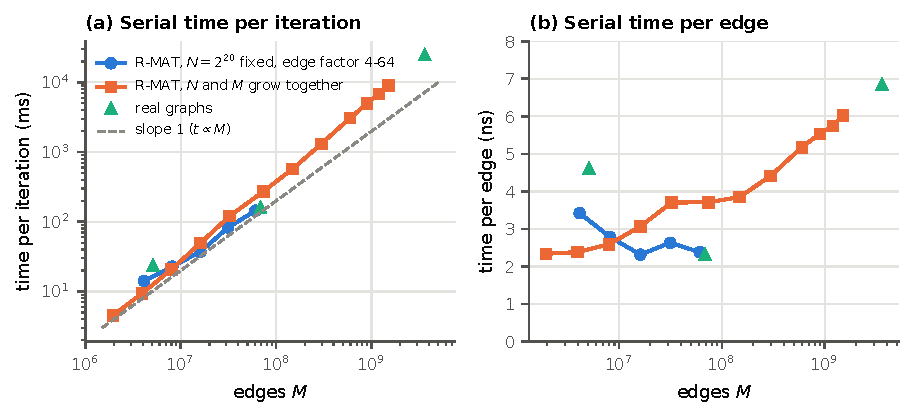
\includegraphics[width=\textwidth]{figures/serial_scaling.pdf}
\caption{Serial program, one core. (a)~Time per iteration against the number of edges for three families. (b)~The
same time divided by $M$.}
\label{fig:serial}
\end{figure}

\begin{table}[tb]
\centering\small
\caption{Serial time per iteration (median of 3 repetitions of 10 iterations).}
\label{tab:serial}
\begin{tabular}{llrrrrr}
\toprule
family & graph & $N$ (M) & $M$ (M) & $M/N$ & ms / iteration & ns / edge \\
\midrule
\tabinput{generated/tab_serial.tex}
\bottomrule
\end{tabular}
\end{table}

To vary both dimensions of the sparse matrix, we vary the number of edges $M$ at a fixed number of vertices $N$
(edge factor 4 to 64), and grow $N$ and $M$ together over three orders of magnitude (R-MAT \code{rmat\_p}$k$, 1.9M
to 1.5G edges). The real graphs are also included (Figure~\ref{fig:serial}, Table~\ref{tab:serial}).

The run time grows linearly with $M$, as the $\Theta(N+M)$ analysis predicts: all points lie close to the slope-1 line
in Figure~\ref{fig:serial}a, from 4.5~ms to 9.0~s. The constant, however, depends on where $x$ fits in the memory
hierarchy:
\begin{itemize}
\item At fixed $N=2^{20}$ (an 8~MB $x$ vector that fits in the L3 cache), the time per edge \emph{falls} from
  \serEFlo\ to \serEFhi~ns as the edge factor grows from 4 to 64. The per-vertex part of the work (the $44N$ bytes of
  the bandwidth model) is spread over more edges.
\item When $N$ and $M$ grow together, the time per edge \emph{rises} from \serRMlo\ to \serRMhi~ns. Up to about
  $N=10^6$ the $x$ vector fits in cache. Beyond $N\approx 1.7\times10^7$ ($8N > 135$~MB, the total L3) almost every
  $x_{\mathrm{src}}$ read goes to DRAM.
\item The real graphs follow the same rule. soc-LiveJournal1 ($x$ = 39~MB, fits in L3) runs at 2.3~ns per edge,
  com-friendster ($x$ = 525~MB) at 6.9~ns per edge, i.e.\ \serFRs~s per iteration.
\end{itemize}
The serial model is therefore $T \approx M \cdot t_e(N) + c\,N$, with $t_e$ between 2.3 and 7~ns depending on whether
$8N$ bytes fit in the cache. This also explains the cache-related effects seen in the parallel runs: splitting a graph
over more ranks shrinks the part of $x$ each rank touches.

\begin{takeaway}
\textbf{Key result.} Serial time grows linearly with the number of edges; the number of vertices sets the constant,
through whether the $8N$-byte vector $x$ fits in the 135~MB L3 cache (2.3~ns per edge) or not (up to 7~ns).
\end{takeaway}

% =====================================================================================================
\section{MPI scaling}
\label{sec:mpi}

\subsection{Strong scaling}

\begin{figure}[tb]
\centering
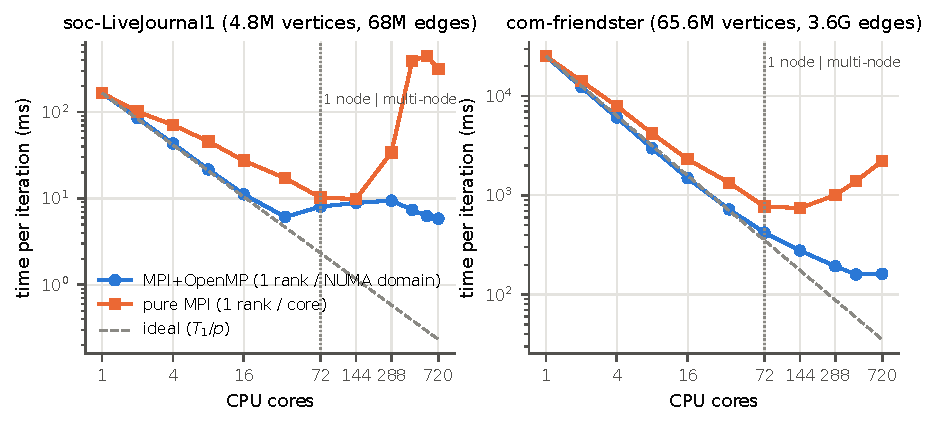
\includegraphics[width=\textwidth]{figures/strong_time.pdf}
\caption{Strong scaling, 1 to 720 cores (10 nodes). Time per iteration of the hybrid layout (one rank per NUMA domain,
36 threads per rank) and of pure MPI (one rank per core) on (a)~soc-LiveJournal1 and (b)~com-friendster. The dotted
line marks one full node.}
\label{fig:strong}
\end{figure}

\begin{figure}[tb]
\centering
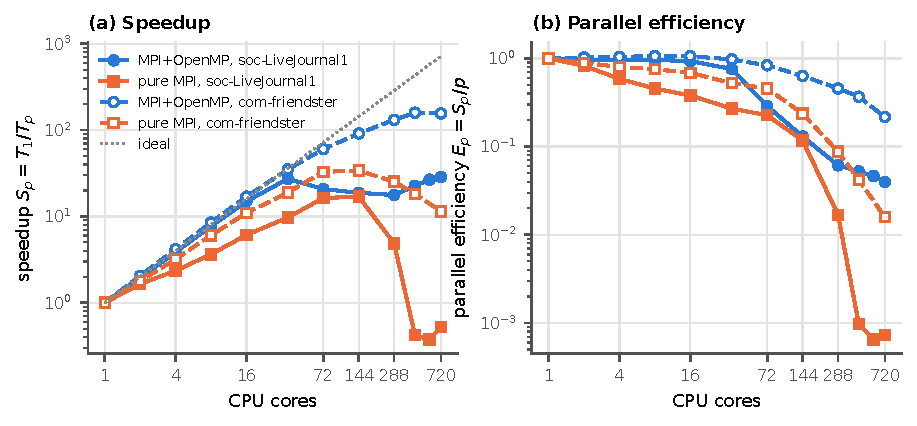
\includegraphics[width=\textwidth]{figures/strong_speedup.pdf}
\caption{Strong-scaling speedup and parallel efficiency, relative to the same program on one core. Filled markers:
soc-LiveJournal1, open markers: com-friendster.}
\label{fig:speedup}
\end{figure}

\begin{table}[tb]
\centering\footnotesize
\setlength{\tabcolsep}{3.6pt}
\caption{Strong scaling: time per iteration $T_p$ (ms), speedup $S_p$ and efficiency $E_p$. ``--'': configuration
did not complete (Section~\ref{sec:transport}).}
\label{tab:strong}
\begin{tabular}{r rrr rrr rrr rrr}
\toprule
& \multicolumn{6}{c}{soc-LiveJournal1} & \multicolumn{6}{c}{com-friendster} \\
\cmidrule(lr){2-7}\cmidrule(lr){8-13}
& \multicolumn{3}{c}{MPI+OpenMP} & \multicolumn{3}{c}{pure MPI} & \multicolumn{3}{c}{MPI+OpenMP} &
\multicolumn{3}{c}{pure MPI} \\
cores & $T_p$ & $S_p$ & $E_p$ & $T_p$ & $S_p$ & $E_p$ & $T_p$ & $S_p$ & $E_p$ & $T_p$ & $S_p$ & $E_p$ \\
\midrule
\tabinput{generated/tab_strong.tex}
\bottomrule
\end{tabular}
\end{table}

Figures~\ref{fig:strong}--\ref{fig:speedup} and Table~\ref{tab:strong} show strong scaling from one core to 10 nodes
for both large real graphs. Within one NUMA domain (up to 36 cores) the hybrid code is close to ideal. com-friendster
reaches $S_{36}=\stFRhyS{36}$ ($E=\stFRhyE{36}$); the slight superlinearity at 2--16 cores is a cache effect (the
threads together hold more of $x$ in their caches). soc-LiveJournal1 reaches $S_{36}=\stLJhyS{36}$. Beyond one node
the two graphs behave differently:
\begin{itemize}
\item \textbf{com-friendster} keeps scaling: \stFRhy{72}~ms on one node, \stFRhy{144}~ms on 2 nodes, \stFRhy{288}~ms
  on 4 nodes and \stFRbest~ms on \stFRbestc\ cores, a speedup of \stFRbestS\ over one core and of 2.6$\times$ over one
  node. Efficiency falls from \stFRhyE{72} (72 cores) to \stFRhyE{288} (288) and \stFRhyE{720} (720), where the time
  stops improving (\stFRhy{720}~ms).
\item \textbf{soc-LiveJournal1} is too small to profit from more than one socket. One iteration takes only
  \stLJhy{36}~ms on 36 cores, which is less than one exchange of its ghost values between nodes. The time stays
  between 6 and 9~ms from 36 to 720 cores. The best value, \stLJbest~ms on \stLJbestc\ cores, is only slightly better
  than one socket.
\end{itemize}

\textbf{Pure MPI} is slower than hybrid at every core count above one, and it collapses on several nodes. On
soc-LiveJournal1 it reaches \stLJmp{144}~ms at 144 ranks but \stLJmp{288}~ms at 288, and 0.3--0.45~s per iteration
at 432--720 ranks: \stLJratio$\times$ slower than hybrid at 432 cores and slower than one core. On com-friendster pure
MPI is fastest at 144 ranks (\stFRmp{144}~ms) and then slows down again, reaching \stFRmp{720}~ms at 720 ranks,
\stFRratio$\times$ the hybrid time. The reasons are analysed next.

\subsection{Weak scaling}

\begin{figure}[tb]
\centering
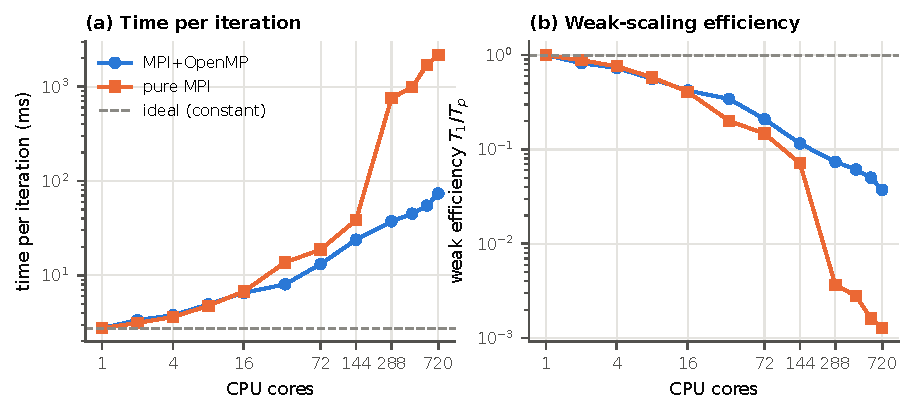
\includegraphics[width=\textwidth]{figures/weak.pdf}
\caption{Weak scaling on R-MAT graphs with $\approx$2M edges per core (\code{rmat\_p}$k$ on $k$ cores; 1.9M edges on 1
core, 1.5G edges on 720 cores). Ideal weak scaling is a constant time.}
\label{fig:weak}
\end{figure}

\begin{table}[tb]
\centering\small
\caption{Weak scaling on \code{rmat\_p}$k$: time per iteration (ms) and weak efficiency $T_1/T_p$.}
\label{tab:weak}
\begin{tabular}{rrr rr rr}
\toprule
& & & \multicolumn{2}{c}{MPI+OpenMP} & \multicolumn{2}{c}{pure MPI} \\
\cmidrule(lr){4-5}\cmidrule(lr){6-7}
cores & $N$ (M) & $M$ (M) & $T_p$ & $T_1/T_p$ & $T_p$ & $T_1/T_p$ \\
\midrule
\tabinput{generated/tab_weak.tex}
\bottomrule
\end{tabular}
\end{table}

For weak scaling the graph grows with the core count (Figure~\ref{fig:weak}, Table~\ref{tab:weak}), from 1.9 million
edges on one core to 1.5 billion edges on 720 cores. The hybrid time per iteration grows from \wkOne~ms to
\wkHy{720}~ms, a weak efficiency of \wkHyE{720}. Three effects cause the growth, and they can be separated:
\begin{enumerate}
\item \textbf{Memory bandwidth within a node} (1--72 cores, efficiency down to \wkHyE{72}). One core draws
  \streamOne~GB/s from memory but 36 cores together only \streamHalf~GB/s (STREAM triad, Figure~\ref{fig:bw}): the
  bandwidth per core drops by half when the socket is full. A bandwidth-bound kernel cannot weak-scale inside a node.
\item \textbf{Cache capacity.} The per-core share of edges is constant, but a rank reads $x$ entries from the whole
  graph. The $x$ vector of \code{rmat\_p}36 (38~MB) still fits in L3; that of \code{rmat\_p}144 (151~MB) does not.
  This is the same effect that raises the serial time per edge (Section~\ref{sec:serial}).
\item \textbf{Communication across nodes} (72--720 cores). After the random relabelling, each rank's ghost set grows
  with the total $N$, so the bytes and the number of partners per rank grow even though the edges per rank stay fixed.
  From 72 to 720 cores the communication time of the hybrid runs grows from 4.8 to 61~ms per iteration while the
  computation time stays at 8--16~ms.
\end{enumerate}
Pure MPI stays within a factor of two of the hybrid code up to 144 ranks (\wkMp{144}~ms). It then jumps to
\wkMp{288}~ms at 288 ranks, the same breakdown as in strong scaling.

\subsection{Impact of communication}
\label{sec:comm}

\begin{figure}[tb]
\centering
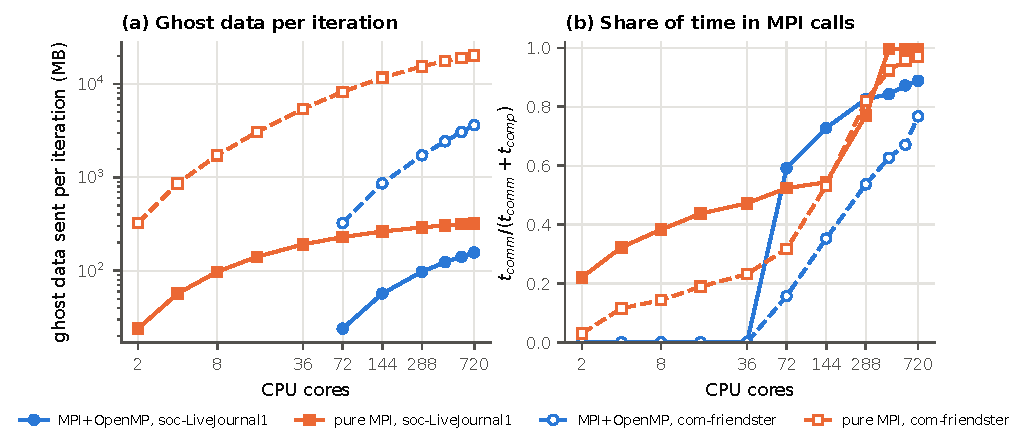
\includegraphics[width=\textwidth]{figures/comm_volume.pdf}
\caption{(a)~Total ghost data sent per iteration, summed over ranks (MB). (b)~Share of the time spent in MPI
calls, $t_{comm}/(t_{comm}+t_{comp})$, from the strong-scaling runs.}
\label{fig:commvol}
\end{figure}

\begin{figure}[tb]
\centering
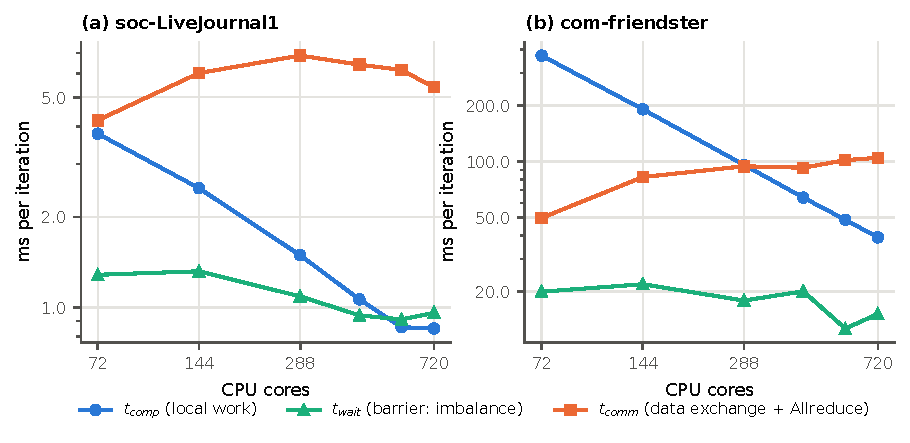
\includegraphics[width=\textwidth]{figures/split_breakdown.pdf}
\caption{Diagnostic \code{--split} runs of the hybrid code: computation, barrier wait (load imbalance and
synchronisation) and pure communication per iteration, from 1 to 10 nodes, for (a)~soc-LiveJournal1 and
(b)~com-friendster.}
\label{fig:split}
\end{figure}

Communication is the part of the problem that limits scaling. The three MPI operations per iteration have very
different costs:
\begin{itemize}
\item the two \code{MPI\_Allreduce} calls move one double each. They cost only latency, and they act as global
  synchronisation points;
\item the \textbf{ghost exchange} moves all the data. Its volume (Figure~\ref{fig:commvol}a) is set by the
  number of ghost vertices. The hybrid layout sends fewer bytes than pure MPI at the same core count: 2--10$\times$ fewer for
  soc-LiveJournal1 and 6--26$\times$ fewer for com-friendster.
  With 36 threads per rank, the 36 cores share one copy of each ghost value, whereas 36 separate ranks would each
  receive their own copy. Allgather would be far worse: on 288 ranks it moves 11~GB per iteration for
  soc-LiveJournal1, against \dzLJbyteG~MB with the ghost exchange (Table~\ref{tab:design}).
\end{itemize}

The share of time spent in MPI calls (Figure~\ref{fig:commvol}b) grows with the number of ranks and exceeds
one half for every multi-node configuration of soc-LiveJournal1. The \code{--split} runs (Figure~\ref{fig:split})
separate waiting from moving data. For com-friendster on 72 cores, an iteration spends \spFRcomp{72}~ms computing,
\spFRwait{72}~ms waiting at barriers and \spFRcomm{72}~ms moving data. On 720 cores computation has dropped to
\spFRcomp{720}~ms, roughly in proportion to the cores, but the data exchange has \emph{grown} to \spFRcomm{720}~ms.
The crossover is at about 288 cores, which matches where the strong-scaling efficiency drops below 0.5. The barrier
wait stays small (15--22~ms) because the edge partition balances the work: load imbalance is not the limit,
communication is.

Even within one node, going from one rank (36 cores) to two ranks (72 cores) makes soc-LiveJournal1 slower
(\stLJhy{36} $\rightarrow$ \stLJhy{72}~ms). The two ranks exchange their ghost values through shared memory, and this
costs \spLJcomm{72}~ms per iteration, more than the \spLJcomp{72}~ms of computation it saves. On Vanda the
single-copy (CMA) mechanism of the shared-memory transport is not permitted, so every message is copied twice through
a shared buffer.

\subsection{Why pure MPI breaks down: TCP between nodes}
\label{sec:transport}

The node's RDMA network adapters are Intel \code{irdma} devices (iWARP/RoCE). The OpenMPI 4.1.8 module on Vanda is
built without UCX, and its \code{openib} BTL is disabled for these devices by default. We forced it on
(\code{--mca btl self,vader,openib --mca btl\_openib\_allow\_ib 1}, experiment E9). Every such run failed at start-up
on 2--10 nodes with ``No OpenFabrics connection schemes reported that they were able to be used'' followed by
``unable to reach each other''. Inter-node MPI messages on Vanda therefore go through the kernel TCP stack
(\code{btl tcp}), with its per-message latency and per-connection socket buffers.

With TCP, the cost of the ghost exchange depends strongly on the number of messages, not only on the bytes. In a
random-like graph almost every rank has ghost vertices on almost every other rank, so the exchange consists of about
$P(P-1)$ messages per iteration: 380 for the 20 ranks of hybrid on 10 nodes, but about 83,000 for 288 pure-MPI ranks
and 518,000 for 720. This is what we see:
\begin{itemize}
\item at 288 ranks on 4 nodes, the allgather (a ring/recursive-doubling collective with $O(P)$ messages per rank)
  beats the ghost exchange on com-friendster (682 vs 1045~ms with the edge partition) despite sending 10$\times$
  more bytes
  (Table~\ref{tab:design});
\item pure MPI on soc-LiveJournal1 jumps from 10~ms (144 ranks) to 34~ms (288) and 0.3--0.45~s (432--720): almost all
  of it is $t_{comm}$ (about 20~s of the 20~s total at 432 ranks);
\item with 576 and 720 ranks, some pure-MPI runs failed with ``\code{mca\_btl\_tcp\_recv\_blocking ... Connection reset
  by peer}''. Several later runs in the same job then failed as well. These configurations were rerun in a separate
  job; any that never completed are shown as ``--''.
\end{itemize}
The hybrid layout avoids the problem because it uses 36$\times$ fewer ranks. It sends fewer bytes, and above all it
sends about $36^2$ times fewer messages and opens 1,300$\times$ fewer TCP connections. On this cluster the
MPI+OpenMP design is therefore not just faster but the only one that scales beyond a few nodes. An MPI library with
RDMA support (e.g.\ an HPC-X/UCX build) would lower the per-message cost, but it would not change the $P^2$ growth of
the message count.

\begin{takeaway}
\textbf{Key result.} The hybrid code scales com-friendster to a speedup of \stFRbestS\ on \stFRbestc\ cores, while
soc-LiveJournal1 is too small to gain beyond one socket. Weak efficiency at 720 cores is \wkHyE{720}. In both cases the
ghost exchange is what grows, and over TCP its cost follows the number of messages ($\approx P^2$), so pure MPI
collapses above 144 ranks.
\end{takeaway}

% =====================================================================================================
\section{MPI+X}
\label{sec:mpix}

\subsection{X = OpenMP: threads, ranks and design choices}

\begin{figure}[tb]
\centering
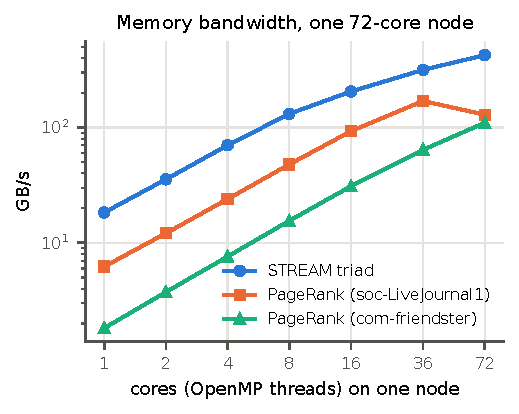
\includegraphics[width=0.52\textwidth]{figures/bandwidth.pdf}
\caption{Memory bandwidth on one node: STREAM triad and the effective bandwidth of the PageRank iteration (hybrid code)
for 1 to 72 cores.}
\label{fig:bw}
\end{figure}

\begin{figure}[tb]
\centering
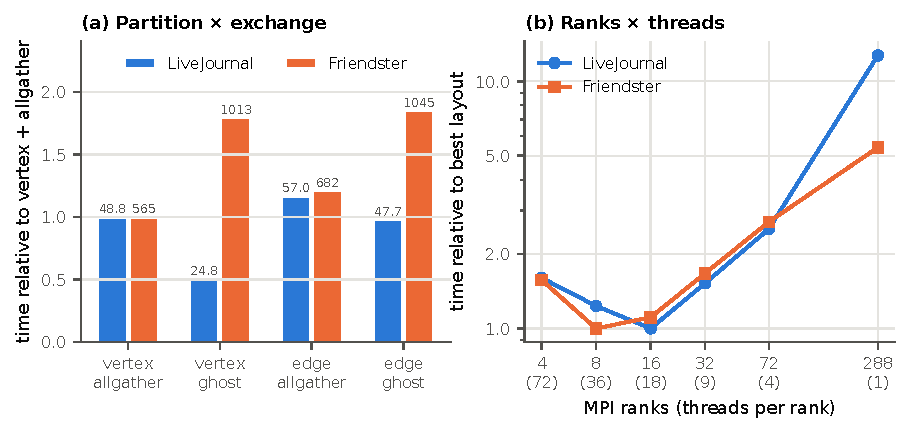
\includegraphics[width=\textwidth]{figures/design.pdf}
\caption{(a)~The four partition and exchange combinations on 288 pure-MPI ranks (4 nodes), relative to the vertex
partition with allgather; the bar labels give ms per iteration. (b)~288 cores split into different numbers of
ranks and threads.}
\label{fig:design}
\end{figure}

\begin{table}[tb]
\centering\small
\caption{Partition and exchange methods on 288 ranks (4 nodes, pure MPI). Times in ms per iteration; the bytes are
the total sent per iteration over all ranks.}
\label{tab:design}
\begin{tabular}{lll rrr rr}
\toprule
graph & partition & exchange & $T$ & $t_{comp}$ & $t_{comm}$ & imbalance & MB / iteration \\
\midrule
\tabinput{generated/tab_design.tex}
\bottomrule
\end{tabular}
\end{table}

\paragraph{OpenMP within a node.} OpenMP threads parallelise the two vertex loops; the SpMV loop uses a dynamic
schedule with chunks of 512 rows, so that threads that hit long rows do not hold up the others. Figure~\ref{fig:bw}
compares the effective bandwidth of the iteration with STREAM. For soc-LiveJournal1 the iteration reaches
\prLJbw{36}~GB/s on one socket, more than half of STREAM (\streamHalf~GB/s): $x$ fits in the L3 cache, so most of the
irregular reads hit cache. com-friendster reaches \prFRbw{72}~GB/s on the full node, a quarter of STREAM
(\streamFull~GB/s), because each random $x$ read moves a full cache line from DRAM. Both curves bend where STREAM bends:
the thread level is limited by memory bandwidth, which is why the hybrid code puts exactly one rank on each socket's
memory.

\paragraph{Ranks $\times$ threads.} On 288 cores (Figure~\ref{fig:design}b) the best split for both graphs is
8 to 16 ranks with 36 or 18 threads, i.e.\ one or two ranks per NUMA domain. Fewer ranks (4$\times$72 threads) put
threads on the remote socket's memory. More ranks increase the communication, up to 13$\times$ the best time for
soc-LiveJournal1 with 288 single-thread ranks.

\paragraph{Partition and exchange.} Table~\ref{tab:design} compares the four combinations on 288 ranks. The edge
partition fixes the load imbalance (\dzLJimbV\ $\rightarrow$ \dzLJimbE\ on soc-LiveJournal1,
\dzFRimbV\ $\rightarrow$ \dzFRimbE\ on com-friendster) and reduces the com-friendster computation time from
\dzFRcompV\ to \dzFRcompE~ms. The ghost exchange cuts the bytes by 10--40$\times$. As discussed in
Section~\ref{sec:transport}, with pure MPI over TCP the message count matters more than the bytes, so on
com-friendster the allgather is faster at this rank count. With the hybrid layout the rank count stays small and the
ghost exchange is the better choice. All scaling runs therefore use the edge partition with the ghost exchange.

\subsection{X = CUDA: one GPU}

\begin{figure}[tb]
\centering
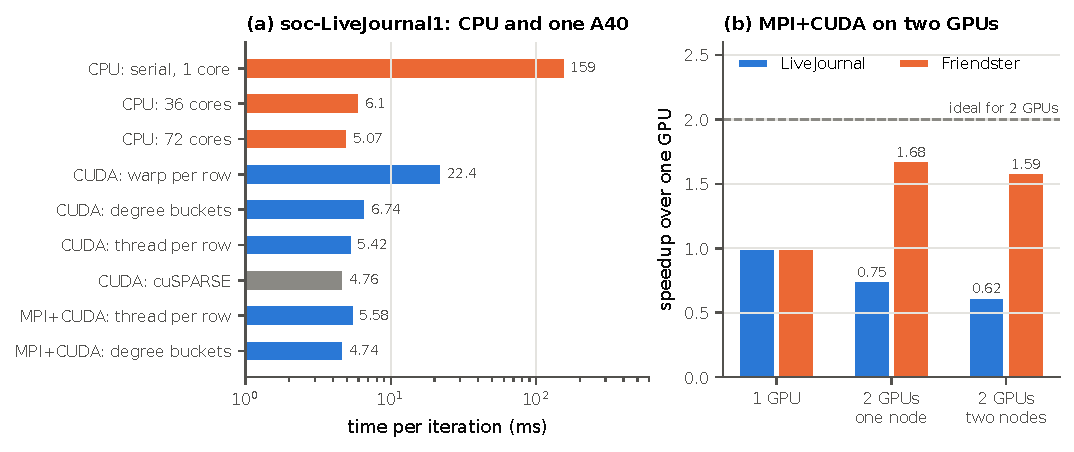
\includegraphics[width=\textwidth]{figures/gpu.pdf}
\caption{(a)~soc-LiveJournal1 time per iteration on CPU cores and on one A40 GPU (four SpMV kernels). (b)~MPI+CUDA speedup with two GPUs on one node and on two nodes.}
\label{fig:gpu}
\end{figure}

\begin{table}[tb]
\centering\small
\caption{Single-GPU kernels on soc-LiveJournal1 (one A40, median of 5$\times$50 iterations): time per iteration,
effective bandwidth $B$ and $B$ as a fraction of the 696~GB/s peak.}
\label{tab:gpu}
\begin{tabular}{lrrr}
\toprule
SpMV kernel & ms / iteration & $B$ (GB/s) & of peak \\
\midrule
\tabinput{generated/tab_gpu.tex}
\bottomrule
\end{tabular}
\end{table}

On one A40 (Table~\ref{tab:gpu}, Figure~\ref{fig:gpu}a), the simple thread-per-row kernel is the fastest of our
kernels (\gpuThr~ms). The warp-per-row kernel is 4$\times$ slower (\gpuWarp~ms) because the median row has only a
handful of in-edges, so most of the 32 lanes idle. The degree-bucket kernel (\gpuHyb~ms) helps the few very long rows
but pays for a second level of indirection through the bucket lists. cuSPARSE, used only as a reference, reaches
\gpuCusp~ms, 12\% faster than our best kernel.

Compared with the CPU, one A40 runs soc-LiveJournal1 \gpuVsSerial$\times$ faster than one core but only about as fast
as one 36-core socket (\gpuThr\ vs \stLJhy{36}~ms), and 1.5$\times$ faster than a full node (\stLJhy{72}~ms). For
com-friendster (MPI+CUDA, one GPU) one iteration takes \mgFRone~ms, which is \emph{slower} than one CPU node
(\stFRhy{72}~ms). The GPU is
\emph{not} limited by its arithmetic. We measured its memory system with \code{tools/gpu\_bw.cu}: a device-to-device
copy reaches \gpuCopy~GB/s and a STREAM triad \gpuTriad~GB/s, but a random gather $y_i = x_{\mathrm{idx}_i}$, the
access pattern of the SpMV, reaches only \gpuGather~GB/s. The GPU moves memory in 32-byte sectors and its 6~MB L2 cannot
hold the 39~MB $x$ vector, so each 8-byte random read costs a full sector from DRAM. The CPU, in contrast, keeps the
whole $x$ of soc-LiveJournal1 in its 135~MB of L3. Our best kernel reaches \gpuThrbw~GB/s of effective bandwidth (27\% of the peak). This is above the
random-gather probe, presumably because the in-edges of a vertex are stored sorted, so neighbouring reads sometimes
share a sector. This is why the GPU
gains only a small factor over a CPU socket: both are bound by irregular memory access, and here the GPU's bandwidth
advantage over the CPU's cache is small.

\subsection{MPI+CUDA: multiple GPUs}

The MPI+CUDA program was run with two GPUs on one node and with one GPU on each of two nodes
(Figure~\ref{fig:gpu}b). On com-friendster, two GPUs give a speedup of \mgFRS\ on one node
(\mgFRone\ $\rightarrow$ \mgFRtwo~ms) and \mgFRSx\ across two nodes (\mgFRxn~ms). The computation halves exactly
(\mgFRcompone\ $\rightarrow$ \mgFRcomp~ms per GPU), and the rest is the ghost exchange through the host: \mgFRcommone~ms
of MPI on one node, \mgFRcommtwo~ms over TCP between nodes, plus \mgFRstage~ms of host--device copies. On
soc-LiveJournal1 one GPU needs only \mgLJone~ms per iteration, less than the exchange itself, so two GPUs are
\emph{slower} (\mgLJtwo\ and \mgLJxn~ms). This is the same lesson as on the CPU: distributing pays off only when the
local work per iteration exceeds the cost of one exchange. Vanda's GPU queue allows at most two GPUs per job, so
larger GPU counts could not be tested.

\begin{takeaway}
\textbf{Key result.} OpenMP inside a socket is limited by memory bandwidth, so one rank per NUMA domain is the best
layout. One A40 GPU matches one 36-core socket on soc-LiveJournal1: its random-gather bandwidth (\gpuGather~GB/s), not
its arithmetic, sets the speed. Two GPUs help only when the local work exceeds one exchange (com-friendster:
\mgFRS$\times$).
\end{takeaway}

% =====================================================================================================
\section{Discussion}
\label{sec:disc}

\paragraph{Conclusions about the data.} On web-Google the PageRank is highly concentrated: the top 0.1\% of pages
hold 11.4\% of the total rank, the top 1\% 27.1\% and the top 10\% 56.8\%. PageRank is strongly but not perfectly
correlated with in-degree (Spearman $\rho=0.85$), and 88 of the 100 highest-ranked pages are also among the 100 pages
with most in-links. The others rank high because they are linked from important pages, not from many pages. For
example, the page ranked 7th has only the 23rd largest in-degree. The 161,168 pages without in-links all share the
minimum score $(1-d)/N + d\delta/N = 2.46\times10^{-7}$, about a fifth of the uniform value $1/N$. The iteration
converges geometrically: the residual falls by a factor of about $0.85$ per iteration, as the damping factor bounds
it, and reaches $10^{-10}$ after \valIters\ iterations.

For the computation, the properties that matter are those of Section~\ref{sec:data}. The data sets differ mainly in
whether the $x$ vector fits in the CPU cache (web-Google and soc-LiveJournal1: yes; com-friendster and the large R-MAT
graphs: no), and in the ratio of local work to communication. com-friendster has 55 edges per vertex: on 144 cores it processes 34 edges per received ghost value,
against 10 for soc-LiveJournal1, which is why it keeps scaling to
432 cores while soc-LiveJournal1 stops at one node. The heavy-tailed degree distribution makes the edge partition
necessary: with a vertex partition, the slowest rank of soc-LiveJournal1 on 288 ranks has 8.6$\times$ the average work.

\paragraph{How the problem was parallelised.}
\begin{itemize}
\item \emph{Between nodes and sockets (MPI):} a 1D row partition by edges, so every rank has the same SpMV work, and a
  precomputed ghost exchange, so every rank receives only the $x$ values it needs. The partition and the
  communication pattern are computed once and reused in every iteration.
\item \emph{Within a socket (OpenMP):} the vertex loops are split over threads that share the rank's memory, so the
  36 cores of a socket share one copy of the ghost values and need no messages among themselves.
\item \emph{On the GPU (CUDA):} one thread per row for the SpMV, and the vectors stay on the GPU. Several kernels were
  compared, and the measured memory probes explain their speed.
\end{itemize}

\paragraph{Which parts need the most communication.} The ghost exchange of $x$ in every iteration needs by far the
most communication: all the data volume, and $O(P^2)$ messages in a random-like graph. The two all-reduces carry only
one number each, but they synchronise all ranks twice per iteration, which is where the barrier wait in
Figure~\ref{fig:split} is paid. Loading and partitioning need no communication beyond a broadcast of the bounds,
because every rank reads its own slice of the file. In our measurements the ghost exchange takes more time than the
computation for every multi-node configuration of soc-LiveJournal1, and for com-friendster from about 288 cores.

\paragraph{Limitations.} (i)~Inter-node MPI ran over TCP; an RDMA-capable MPI would shift all multi-node curves down,
and should help pure MPI most. (ii)~We did not reorder the vertices (e.g.\ by graph partitioning or locality-aware
relabelling). Such reordering would reduce the number of ghost vertices and is the most promising way to improve
scaling further. (iii)~GPU runs are limited to two GPUs per job on Vanda. (iv)~A few pure-MPI configurations at 576
and 720 ranks did not complete because of TCP connection resets; they are reported as missing, not estimated.

% =====================================================================================================
\section*{Declaration of AI use}
We used an AI assistant (Claude, by Anthropic) during this project for code review and debugging of the job scripts
and timing code, for writing the experiment scripts (\code{jobs/final}), the bandwidth probes and the analysis and
plotting scripts, and for drafting and editing parts of this report. All experiments were designed, run and checked by
us on Vanda. Every number in the report comes from our own measurement files, and we reviewed all code and text.

\section*{Source code and reproduction}
The repository contains the source (\code{src/}), the preprocessing and generator tools (\code{tools/}), the PBS job
scripts used for every result (\code{jobs/final/}), the raw result files (\code{results\_final/}) and the script that
builds all figures and tables (\code{tools/make\_report.py}). \code{README.md} describes how to build, download
the data, submit the jobs and regenerate this report.

\begin{thebibliography}{9}\small
\bibitem{pagerank} L.~Page, S.~Brin, R.~Motwani, T.~Winograd. The PageRank citation ranking: bringing order to the
  web. Stanford InfoLab technical report, 1999.
\bibitem{snap} J.~Leskovec, A.~Krevl. SNAP Datasets: Stanford large network dataset collection.
  \url{http://snap.stanford.edu/data}, 2014.
\bibitem{rmat} D.~Chakrabarti, Y.~Zhan, C.~Faloutsos. R-MAT: a recursive model for graph mining. SIAM International
  Conference on Data Mining, 2004.
\bibitem{graph500} Graph500 benchmark specification, \url{https://graph500.org}.
\bibitem{stream} J.~D.~McCalpin. Memory bandwidth and machine balance in current high performance computers. IEEE
  TCCA Newsletter, 1995.
\end{thebibliography}

\end{document}
